\chapter{文獻探討}


\section{品牌的定義}

根據各學者指出品牌的定義如以:

美國行銷學會(American Marketing Association,AMA)
對品牌的定義為\cite{AMA}:名稱 (Name)詞語(Term) 標記(Sign)象徵(Symbol )設計(design)

Sappington and Wernerfelt (1985) 提出品牌名稱是企業的一項貴重資產,可以提升消費者對於產品的需求性,減少顧客的不確定感,且品牌名稱也被當成是對公司產品的品質保證\cite{Sappington}。

Farquhar (1989) 品牌是一個名稱、符號、設計或標誌,可以使一個產品增加功能利益還有以外的價值\cite{Farquhar}。



Rao and Ruekert (1994)品牌對於消費者而言是屬於產品的一部分,可視為傳遞產品品質訊息的媒介,而且往往是消費者購買決策的重要考量因素之一,具有增加產品價值的功能,而且可以提供產品一定的品質保證,降低消費者的搜尋成本及知覺風險\cite{Rao}。 

Boyd, Walker, 和 Larreche (1995)認為品牌的構成,成分一般可以細分為\cite{Boyd} :
\begin{enumerate}
\item 品名(brand name):可以發聲唸出的部分。
\item 品牌標誌(brand mark):不能以言語表達的部分,例如符號、設計或獨特的包裝。 
\item 商標(trademark):法律上,專屬於某一個賣方的品牌或品牌的某部分。
\end{enumerate}

另外,根據 Laforet 和 Saunders (1994) 的實證研究,歸納出三種品牌導向,六種品牌策略,這三種品牌導向所引發出的六個策略為\cite{Laforet}:
\begin{enumerate}
\item 企業品牌導向

1.企業品牌策略:直接採用企業名稱作為產品品牌名稱。 

2.部門品牌策略:當企業跨足不同市場,單一企業名稱不敷使用時,不同部門採用不同附屬名稱 (subsidiary name) 作為產品品牌名稱
\item 產品品牌導向

1.個別品牌策略:各產品專屬品牌,不刻意突顯企業名稱,但在包裝上某處仍會出現。

2.獨立品牌策略:各產品專屬品牌,但是刻意不揭露企業名稱,不希望消費者知道是哪一家企業製造。
\item 混合品牌導向

1.雙重品牌策略:兩個或更多層級的品牌要素,組合而成產品品牌,而且每個品牌要素的顯著性相等。

2.背書式品牌策略:同樣以兩種品牌要素組成品牌,但企業或家族品牌作為背書之用,新產品的品牌較為顯著。
\end{enumerate}
De Chernatony and McDonald,(1998)出消費者選擇一個品牌時,他們會進行評估實用能力,以及品牌所象徵著的意義\cite{Chernatony1998}。De Chernatony,(2001)品牌被解釋為行為表現、風格、外觀、聲音、信念和態度的服務人員\cite{Chernatony2001}。

 鄒風&孟林明(1997)知覺會受到主觀個人狀態與客觀環境刺激兩種因素影響,詳述如下\cite{鄒風、孟林明}:
\begin{enumerate}
\item 主觀個人狀態:指消費者當前的生理與心理狀態,包括消費者的需要、 期望、過去的經驗、價值觀念、態度、信念與態度等。
\item  客觀環境刺激:指可以設法操縱的環境因素,包括物體大小、色彩、聲 音、位置、店鋪、產品品牌、包裝、價格、推銷、廣告與情境等。
\end{enumerate}

\begin{table}[htb]
\caption{品牌的文獻整理}
\label{tab:PL1}
\centering
%\renewcommand{\arraystretch}{1.2} % 將表格行間距加大為原來的 1.2 倍
%\arrayrulewidth=1pt % 調整線條粗細為 1pt
%\tabcolsep=24pt % 調整欄間距為 24pt
%\begin{document}
\begin{tabular}[t]{|c|p{8.5cm}|p{2.5cm}|} % 第一欄位使用 sans serif 字族
\hline
學者&定義 & 年代 \tabularnewline
\hline
美國行銷學會 & 對品牌的定義為:名稱 (Name)詞語(Term) 標記(Sign)象徵(Symbol )設計(design)&  \tabularnewline
\hline
Sappington and Wernerfelt  &企業的品牌名稱是一個寶貴的資產,可以提升消費者對
於產品的需求性,減少顧客的不確定感,且品牌名稱也被當成是對公司產品的品質保證。& 1985 (施瑩婕(2009)譯) \tabularnewline
\hline
Farquhar &品牌是一個名稱、符號、設計或標誌,可以使一個產品
增加的不僅是功能利益還有功能利益以外的價值。&1989 (施瑩婕(2009)譯) \tabularnewline
\hline
Rao and Ruekert &品牌對於消費者而言是屬於產品的一部分,可視為傳遞產品品質訊息的媒介,而且往往是消費者購買決策的重要考量因素之一,具有增加產品價值的功能,而且可以提供產品一定的品質保證,降低消費者的搜尋成本及知覺風險。&1989(施瑩婕(2009)譯)  \tabularnewline
\hline
 Laforet 和 Saunders&歸納出三種品牌導 :(一)企業品牌導向(二)產品品牌導向(三)混合品牌導向
&1994\tabularnewline
\hline
oyd, Walker, 和 Larreche&認為品牌的構成,成分一般可以細分為:(一)品名(brand name)(二)品牌標誌(brand mark)(三)商標(trademark)&1995\tabularnewline
\hline
De Chernatony and McDonald&出消費者選擇一個品牌時,他們會進行評估實用能力,以及品牌所象徵著的意義&1998
\tabularnewline
\hline
De Chernatony&品牌被解釋為行為表現、風格、外觀、聲音,信念和態度的服務人員。&2001
\tabularnewline
\hline
 鄒風&孟林明&知覺會受到主觀個人狀態與客觀環境刺激兩種因素影響
&1997(王翎幗,2006譯)\tabularnewline
\hline
\end{tabular}
\end{table}

以上學者對於「品牌」的定義可以瞭解,許多學者舉出的品牌定義並不一致,但可以瞭解出品牌是公司無形有力的資產,由以上可看出品牌對公司來說非常的重要不但能提升公司的營運與消費者對公司的認知

\section{品牌知覺}
Aaker (1991) 將消費者對品牌的知覺品質定義為消費者對於某一 項品牌產品整體品質的認為水準,或消費者對在特定目的下相對於其他品牌,對某品牌產品或服務全面品質的主觀滿意程度。\cite{Aaker1991}

kelle(1993)認為品牌認知是指在消費者記憶中較強的品牌聯想與連接。
將品牌知覺的衡量主要分成三種\cite{Keller1993},敘述如下:
\begin{enumerate}
\item 屬性:消費者在消費之餘所認知的品牌是什麼、品牌有什麼。
\item 利益:指消費者個人價值。
\item 態度:指消費者對品牌整體的評價
\end{enumerate}

%Dawar and Parker(1994) 指出消費者挑選產品以品牌聲望為主要考量
%Herbig and Milewica(1996) 正向的品牌聲望有助收益增加。
%Kowallczyk and Pawlish(2002)公司聲望是影響消費者購買的因屬之一。
%Veloutsou and Moutinho(2009)維持和提升公司聲望比強化消費者滿意度更重要
%Priporas and Kamenidou(2011)品牌聲望佈警示品牌保證,也是行銷推廣的利器

keller (1998)提出品牌的意義與功能可以從四種角度來說明\cite{Keller1998}:
\begin{enumerate}
\item 品牌可以用圖案來辨別,可用來與競爭者來區別

\item 品牌一致的保證與承諾,是消費者在購買或使用之前的感覺產品的價值與品質

\item 品牌是可以自我投射形象,品牌個性的傳達

\item 品牌不僅是一組有關產品的定位,代表一致性品質與功能性的集合,也可作為消費者決策購買時的線索
\end{enumerate}
    Keller (1998)亦詳細地指出,品牌權益實包含\cite{Keller1998}:
\begin{enumerate}
\item 品牌鮮明度 (Brand Salience):可能會影響消費的判別難易度
\item 品牌績效 (Brand Performance):可以滿足消費者所需功能
\item 品牌形象 (Brand Image):在消費者心中產生對品牌抽象整體概念
\item 品牌判斷 (Brand Judgment) :消費者對於品牌理性層面的判定
\item 品牌情感 (Brand Feeling):消費者對品牌情感的概念與特性,或是社會認可的特徵
\item 品牌共鳴 (Brand Resonance):與消費者品牌關係的最高層次,是由品牌情感到具體行動購買的具體表現,例如主動參與及重複購買的行為忠誠度。
\end{enumerate}
  
Aaker (1996)認為品牌權益可分為\cite{Aaker1996}:
\begin{enumerate}
\item 品牌知名度 (Brand Awareness)
\item 品牌忠誠度 (Brand loyalty) 
\item 品牌知覺品質 (Brand perceived quality) 
\item 品牌聯想 (Brand Association)
\item 其他品牌專屬資產 (Brand Speciality Asset) 。
\end{enumerate}


%\begin{figure}[htbp]
%\centering 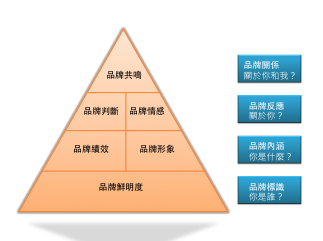
\includegraphics[%
 % width=13cm,keepaspectratio]{images/keller2008}
%\caption{\label{fig:keller}來自keller2008}
%(資料來源:本研究整理)
%\end{figure}



\begin{table}[htb]
\caption{品牌知覺的文獻整理}
\label{tab:PL2}
\centering
%\renewcommand{\arraystretch}{1.2} % 將表格行間距加大為原來的 1.2 倍
%\arrayrulewidth=1pt % 調整線條粗細為 1pt
%\tabcolsep=24pt % 調整欄間距為 24pt
%\begin{document}
\begin{tabular}[t]{|c|p{8.5cm}|p{2.5cm}|} % 第一欄位使用 sans serif 字族
\hline
學者&定義 & 年代 \tabularnewline
\hline
Aaker & 將消費者對品牌的知覺品質定義為消費者對於某一 項品牌產品整體品質的認為水準,或消費者對在特定目的下相對於其他品牌, 對某品牌產品或服務全面品質的主觀滿意程度。& (1991)  \tabularnewline
\hline
kelle&將品牌知覺的衡量主要分成三種,敘述如下:屬性,利益,態度& 1993 \tabularnewline
\hline
Aaker&認為品牌權益可分為:(1)品牌知名度 (Brand Awareness)、(2)品牌忠誠度 (Brand loyalty) 、(3)品牌知覺品質 (Brand perceived quality) 、(4)品牌聯想 (Brand Association)、(5)其他品牌專屬資產 (Brand Speciality Asset) &1996。\tabularnewline
\hline
Keller&提出品牌的意義與功能可以從四種角度來說明:品牌可以用圖案來辨別,品牌一致的保證與承諾,品牌是可以自我投射形象,品牌不僅是一組有關產品的定位。&1998 \tabularnewline
\hline
Keller&指出品牌權益實包含:品牌鮮明度 (Brand Salience),品牌績效 (Brand Performance),品牌形象 (Brand Image),品牌判斷 (Brand Judgment),品牌情感 (Brand Feeling),品牌共鳴 (Brand Resonance),例如主動參與及重複購買的行為忠誠度。&1998 \tabularnewline
\hline
\end{tabular}
\end{table}
以上學者對於「品牌知覺」的定義可以瞭解,許多學者舉出的品牌知覺定義可瞭解出,品牌知覺是消費者對於公司 品牌的第一知覺投射的映像,消費者由於品牌知覺好壞所影響一個公司的品牌定位。


\section{消費者行為}
早期的消費者行為通常都以消費者動機來當研究核心,隨著各位學者長年研究下來提出了許多相關理論的模式,但是現在研究後期主要都已決策的過程為主要核心

Pratt(1974)消費者行為是指購買行動,其中購買的行動至 少包括四個因素\cite{Pratt1974}:
\begin{enumerate}
\item 購買主體-購買者本身; 
\item  購買物品或勞務;
\item  購買媒介-現金或支 付的承諾;
\item  決定購買的行動。
\end{enumerate}

Walter&Gordon(1970)指人們在購買、使用產品或服務時的相關行為\cite{Walter1970}。另一位學者林靈宏(2000)將消費者個體視為一個心理單位,消費者的價 值觀、知覺、學習、人格、動機、經驗、記憶、 認知、態度及涉入程度都會影響消費行為\cite{林靈宏}。

Schiffman&Kanuk(2003)瞭解消費者是如何進行決策,以支配可得資源 (時間、金錢、努力)於各種消費項目。這些決策 包括購買何種物品 (what)?為何而買 (why)? 何時購買 (when)?在哪裡購買 (where)?多常 購買 (how often)?以及使用 (use) 頻率\cite{Schiffman}。

程信賢(2002)提出了消費者在購買動機上無顯著差異;在人口統計變數中除了性別變數外其餘變數皆具有顯著差異;在購買決策變數之資訊尋求、評估準則、消費實態等變數,均具有顯著差異\cite{程信賢}。

\section{消費者行為理論(Consumer Behavior Theory)}
\subsection{EBK消費者行為定義}
消費者行為可以定義於:消費者在搜尋、評估、購買、使用和處理一項產品、服務、和理念(ideas)時表現的行為。
\begin{figure}[htbp]
\centering 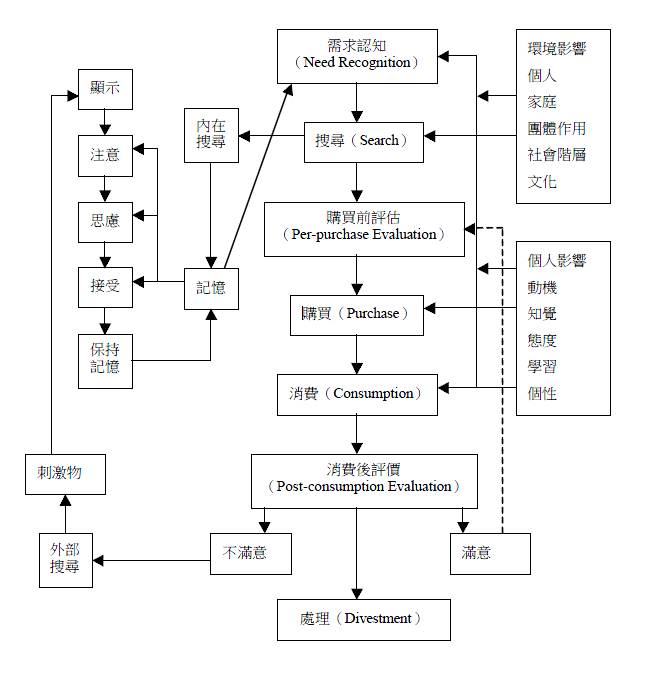
\includegraphics[%
  width=16cm,keepaspectratio]{images/ConsumerBehaviorTheory}
\caption{\label{fig:ConsumerBehaviorTheory}Engel, Blackwell and Kollat(1993) 汪澤普(2005)整理}
%(資料來源:本研究整理)
\end{figure}

消費者決策行為模式有好幾種,其中較為完整且具系統性的模式架構的
是EKB Model(Engle, Kollat & Blackwell Model)。
Engel, Blackwell, and Kollat 等學者在 1968 年從消費者行為理論中,發展出了 EKB 模型 (Engel-Kollat-Blackwell Model, EKB Model)(汪澤普2005譯)
在 EKB 模型中,可以分為四大部分\cite{汪澤普}:
\begin{enumerate}
\item 輸入(Input):消費者所接受的外界訊息,其主要來自於兩方面:一是非行銷來源,如大眾傳播媒體或人際溝通管道;二是從行銷來源,如廠商的行銷活動。
\item 資訊處理(Information Processing):資訊處理是經由刺激的接受、中斷與記
憶的儲存和稍後取用的過程,可分為展露(Exposure)、注意(Attention)、理
解(Comprehension)、接受(Acceptance)及保留(Retention)等五個步驟。
\item 決策過程(Decision Process):決策過程可分為五個階段,是EKB模型中最主要的部分,此五個階段雖然是線性的過程,但卻可以反覆地回到之前的階段(Zellwegger 1997),此五個階段敘述如下:

a. 需求確認(Problem Recognition):是消費者決策過程中的第一個階段,當消費者認知到現實與理想狀態存在著差距時,就會意識到需求的存在,而這些需求有可能會被外部的或內部的因素所觸發,比如:廠商的促銷活動或者是個人的經濟狀況提升等等。

b. 資訊搜尋(Information Search):消費者在確認了需求動機後,就會開始搜尋資訊,搜尋的範圍包括了記憶中的知識及外部的環境,前者稱為內部搜尋,後者則稱為外部搜尋。

c. 選擇評估(Alternative Evaluation):當消費者取得了足夠的資訊後,即 會對可能的選擇方案加以分析與評估,來做為後續制訂購買決策的依據。

d. 購買(Purchase):經過審慎的分析與評估後,消費者會從選擇方案中選 擇其一購買;消費者在這階段中,也必須決定從何處以及如何購買。

e. 購後行為(Post-purchase):消費者在使用或消費所選擇的商品或服務後,會對其做出評估,以做為下此購買的參考。

\item 影響決策變數(Variables Influence Decision Process):影響決策過程的變數可分為兩部分:一為環境因素,包括文化、社會階層、個人影響、家庭與情境 等因素;二為個人差異,包括消費者資源、動機與涉入、知識、態度、人格、 價值觀與生活形態。
\end{enumerate}



\begin{table}[htb]
\caption{消費者決策的文獻整理}
\label{tab:PL3}
\centering
%\renewcommand{\arraystretch}{1.2} % 將表格行間距加大為原來的 1.2 倍
%\arrayrulewidth=1pt % 調整線條粗細為 1pt
%\tabcolsep=24pt % 調整欄間距為 24pt
%\begin{document}
\begin{tabular}[t]{|c|p{8.5cm}|p{2.5cm}|} % 第一欄位使用 sans serif 字族
\hline
學者&定義 & 年代 \tabularnewline
\hline
Pratt1974 &消費者行為是指購買行動,其中購買的行動至 少包括四個因素:(1)買主體-購買者本身; (2)購買物品或勞務;(3)購買媒介-現金或支 付的承諾;(4)決定購買的行動。
& 1974  \tabularnewline
\hline
Walter&指人們在購買、使用產品或服務時的相關行為。& 1970 \tabularnewline
\hline
林靈宏&將消費者個體視為一個心理單位,消費者的價 值觀、知覺、學習、人格、動機、經驗、記憶、 認知、態度及涉入程度都會影響消費行為 &2000。\tabularnewline
\hline
Schiffman&Kanuk&瞭解消費者是如何進行決策,以支配可得資源 (時間、金錢、努力)於各種消費項目。這些決策包括購買何種物品 (what)?為何而買 (why)? 何時購買 (when)?在哪裡購買 (where)?多常 購買 (how often)?以及使用 (use) 頻率。&2003 \tabularnewline
\hline
Engel, Blackwell, and Kollat &EKB 模型中,可以分為四大部分:輸入(Input),資訊處理(Information Processing),決策過程(Decision Process),影響決策變數(Variables Influence Decision Process)&1968  \tabularnewline
\hline
\end{tabular}
\end{table}

\subsection{影響消費行為的心理因素}
消費者行為可以定義於:消費者在搜尋、評估、購買、使用和處理一項產品、服務、和理念(ideas)時表現的行為\cite{林靈宏}。
\begin{figure}[htbp]
\centering 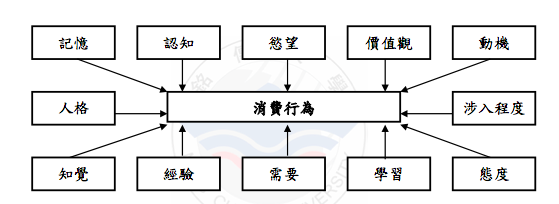
\includegraphics[%
 width=13cm,keepaspectratio]{images/影響消費行為的心理因素}
\caption{\label{fig:影響消費行為的心理因素}林靈宏 (2000),消費者行為學,台北:五南圖書出版公司。}
%(資料來源:本研究整理)
\end{figure}


\subsection{消費者決策行為在傳統市場與網路市場中的差異}
Bulter and Peppard(1998) 以EKB 型中的消費者決策過程,來比較實體市場(Marketplace)與網路市場(Marketspace)中對消費者不同的影響,以及行銷人員在面對此兩種市場時,在行銷活動上的差異,以下就以此五個階段的決策過程來分別說明\cite{Bulter1998}:
\begin{enumerate}
\item  需求確認:此階段主要的行銷策略,在於發 展能預測甚或刺激消費者需求的傳播能力。
\item  資訊搜尋:此階段的重心,在於資訊的來源,主要的行銷策略,是要吸引正在搜尋資訊的消費者(information-seeking consumer),並且提供他們所需要的資訊。
\item  選擇評估:此階段首要的行銷策略,在於了 解消費者評估產品的標準、消費者的偏好,以及其他競爭者的行銷策略。
\item  購買:認為,此階段的核心問題,在於消費者為 何要購買,消費者將在此階段中決定去何處購買,以及如何購買;而訂購、付款與遞送流程的完善,是這階段中最主要的策略任務,行銷人員要能建立 起讓消費者感到舒適的購買環境與購買方式。
\item  購後行為:認為,行銷人員需在此階段了解消費 者在購買後的行為,以發展顧客關係及消費者忠誠度。
\end{enumerate}

\begin{figure}[htbp]
\centering 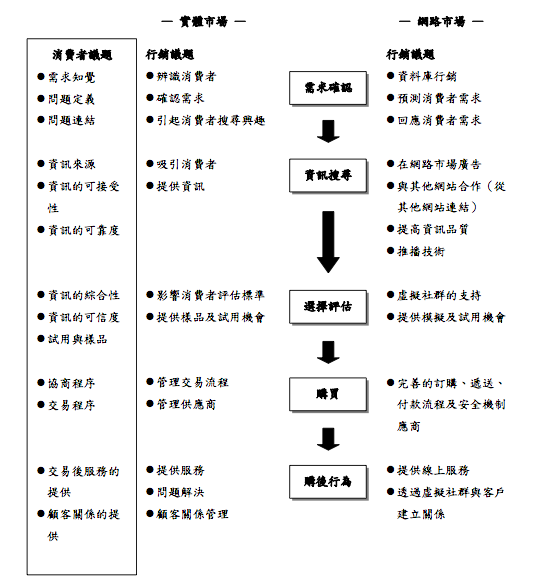
\includegraphics[%
  width=16cm,keepaspectratio]{images/Difference}
\caption{\label{fig:ConsumerBehaviorTheory}Bulter and Peppard(1998) 汪澤普(2005譯)}
%(資料來源:本研究整理)
\end{figure}


\section{影響消費購買意願}
\subsection{購買意願之購買決策過程}
Engel, et al (2001) 認為,消費者決策過程的五個重要階段如圖~\ref{fig:Engel}
\begin{enumerate}
\item 問題認知

購物過程開始時於消費者觀察自身需求與問題來源的認知 ;消費者在問題認知方面會受到外在因素影響(文化,人口統計變數,慘考群體)與個人因刺激,引起消費者產生動機

\item 尋求

消費者在確定自己本身所需後,會根據自身所需或是問題來尋求相關資訊,以進行購物決策。一般的消費者收集資訊通常都分為兩種來源,內部搜尋與外部搜尋;消費者,通常會先從自身的記憶中搜尋所需的相關資訊,如過記憶中沒有相關記憶就會改以外部搜尋,獲得協助決策的相關資訊,外部搜尋的資訊如:家人,朋友,廣告,網路等。
           
\item 方案評估

搜尋資料完後,就可以對所需要的選著方案做評估與最後的決策。通常消費者都是透過各項評估的標準與尺度來評定購買的方案。

\item 選擇

經過以上敘述方案評估過程後,消費者會以全部方案中選擇最適合的方案,並購買的行動。

\item 結果 

當消費者購買產品後,因為本身對產品的期望結果與實際使用的結果,兩種之間的感覺受差異。
一般消費者購買的商品使用後心裡的感受主要有三中結果

符合期望:消費者使用購買的產品後的結果表現符合預期的期望,沒有特別好或壞的感覺

非常滿意:消費者使用購買的產品後的結果表現超過預期的期望,導致心裡的感覺很滿意

不滿意:消費者使用購買的產品後的結果表現低於預期的期望,導致心裡的感覺很不滿意的反應
\end{enumerate}

據以上學者所對消費者行為定義,因此可解釋消費者行為分為:消費者在搜尋、評估、購買、使用和處理一項產品、服務、和理念(ideas)時表現的行為。
\subsection{消費者滿意度}
消費者滿意度:

     「消費者滿意度」最早由 Cardozo 於 1964 年所提出以實證研究方式探討顧客預期與實際感受之差 距對滿意度以及滿意度對再購意願之影響。

Fornell(1992)指出消費者滿意度是指顧客在購買產品 或使用服務後主觀性的整體衡量。


Oliver (1977, 1980,1981) 滿意度的基礎框架.是指消費者在購買產品或使用服務前會先產生期望,而在使用產品或服務後,實際效果表現會與先前的期望互相比較,造成滿意程度上的差別,當時實際效果表現高於期望時,稱之為正向,而當實際效果表現低於期望時,稱為負向.當正向值越高即代表滿意度越高,消費者持續購買產品或使用服務的機會交高,而當負向越高即滿意度越低,會減少消費者持續購買產品或使用服務的意願\cite{Oliver1980}。

Turner(2011)則提到,顧客滿意度包含了幾項影響因子,分別為產品(特色、品質、獨特 性 )、與可替代品的價格比較 、 競爭環境、品牌與其產品之間的情感聯繫、與顧客以往的互動所建立的商譽及其他內外在因素(醜聞、政經環境等)。總而言之,消費者滿意度是結合消費者認知及情感的綜合評量結果\cite{Turner2011}。

陳思璇(2011)提出 資訊品質及服務品質顯著地影響重購顧客之滿意度,且顧客滿意顯著地影響重購顧客之再購買意願\cite{陳思璇}。然而,系統品質對重購顧客而言效果並不顯著。另位張倫嚴(2012)產品創新、產品涉入、知覺價值與顧客滿意度間具有顯著正向影響\cite{張倫嚴}。

藍悅真(2012)提出1.品牌形象的「功能性」、「經驗性」能正向預測消費者滿意度的產品滿意。2.品牌形象的「功能性」、「象徵性」能正向預測消費者滿意度的服務滿意。3.品牌形象的「功能性」、「經驗性」能正向預測消費者滿意度的整體滿意。4.品牌形象的「功能性」、「經驗性」能正向預測消費者忠誠度\cite{藍悅真}。

以上學者對於「消費者滿意度」的定義可以瞭解,雖然個學者們沒有一致的定義,但都有提到消費者滿意度度乃建構在購買前消費者對商品與服務的預期與購買獲得的效益認知差異,兩者差距用大時顧客對於滿意與不滿意越明顯。



\begin{figure}[htbp]
\centering 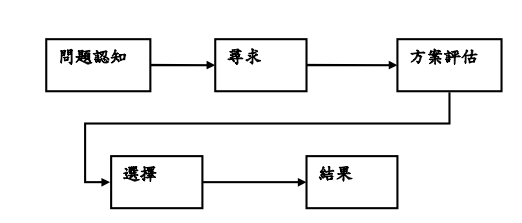
\includegraphics[%
  width=13cm,keepaspectratio]{images/Engel}
\caption{\label{fig:Engel}Engel, et al (2001)}
%(資料來源:本研究整理)
\end{figure}

\begin{table}[htb]
\caption{消費者滿意度的文獻整理}
\label{tab:PL4}
\centering
%\renewcommand{\arraystretch}{1.2} % 將表格行間距加大為原來的 1.2 倍
%\arrayrulewidth=1pt % 調整線條粗細為 1pt
%\tabcolsep=24pt % 調整欄間距為 24pt
%\begin{document}
\begin{tabular}[t]{|c|p{8.5cm}|p{2.5cm}|} % 第一欄位使用 sans serif 字族
\hline
學者&定義 & 年代 \tabularnewline
\hline
 Cardozo & 探討顧客預期與實際感受之差 距對滿意度以及滿意度對再購意願之影響。& 1964  \tabularnewline
\hline
Fornell&指出消費者滿意度是指顧客在購買產品 或使用服務後主觀性的整體衡量。& 1992 \tabularnewline
\hline
Oliver &滿意度的基礎框架.是指消費者在購買產品或使用服務前會先產生期望,而在使用產品或服務後,實際效果表現會與先前的期望互相比較,造成滿意程度上的差別,當時實際效果表現高於期望時,稱之為正向,而當實際效果表現低於期望時,稱為負向.當正向值越高即代表滿意度越高,消費者持續購買產品或使用服務的機會交高,而當負向越高即滿意度越低,會減少消費者持續購買產品或使用服務的意願。&1977, 1980,1981\tabularnewline
\hline
Turner&則提到,顧客滿意度包含了幾項影響因子,分別為產品(特色、品質、獨特 性 )、與可替代品的價格比較 、 競爭環境、品牌與其產品之間的情感聯繫、與顧客以往的互動所建立的商譽及其他內外在因素(醜聞、政經環境等)。總而言之,消費者滿意度是結合消費者認知及情感的綜合評量結果。&2011 \tabularnewline
\hline
\end{tabular}
\end{table}


\begin{table}[htb]
\caption{消費者滿意度的文獻整理}
\label{tab:PL5}
\centering
%\renewcommand{\arraystretch}{1.2} % 將表格行間距加大為原來的 1.2 倍
%\arrayrulewidth=1pt % 調整線條粗細為 1pt
%\tabcolsep=24pt % 調整欄間距為 24pt
%\begin{document}
\begin{tabular}[t]{|c|p{8.5cm}|p{2.5cm}|} % 第一欄位使用 sans serif 字族
\hline
陳思璇&資訊品質及服務品質顯著地影響重購顧客之滿意度,且顧客滿意顯著地影響重購顧客之再購買意願。然而,系統品質對重購顧客而言效果並不顯著。&2011 \tabularnewline
\hline
張倫嚴&產品創新、產品涉入、知覺價值與顧客滿意度間具有顯著正向影響。&2012
\tabularnewline
\hline
藍悅真&1.品牌形象的「功能性」、「經驗性」能正向預測消費者滿意度的產品滿意。2.品牌形象的「功能性」、「象徵性」能正向預測消費者滿意度的服務滿意。3.品牌形象的「功能性」、「經驗性」能正向預測消費者滿意度的整體滿意。4.品牌形象的「功能性」、「經驗性」能正向預測消費者忠誠度。&2012
\tabularnewline
\hline
\end{tabular}
\end{table}

\section{La jolla樂活雅}
\begin{enumerate}
 \item 經營據點:台灣:台北市大安區光復南路446號七樓 
               美國:2231 N. 23rd St. Beaumont, TX 77706

 \item  經營理念:
富紳國際實業有限公司主要從事首飾及貴金屬零售業;擁有為數不少的客戶群。
最初,是由兩位業餘華裔設計師,自行創作手工珠寶藝品,由於設計風格獨特,大受消費者的歡迎及喜愛,總是供不應求。設計師們有鑑於手工飾品無法大量生產,又觀察到,在未來的飾品趨勢中,鈦飾品將取代金銀等貴重金屬,成為高級珠寶設計重要材質,因此決定發展鈦鍺飾品。

以生產設計鈦鍺精品為主的富紳國際,也接受客戶OEM及ODM訂單。舉凡項鍊、手鍊、戒指、袖扣等商品,並供貨給日本、美國等客戶及珠寶精品業者。
另外,富紳國際亦提供客製化服務,承接結合鈦飾品及頂級鑽石之客製化訂單,為消費者
提供獨一無二的商品訂製服務。

發展至今,富紳國際已擁有自己的設計師及協力生產工廠,從來圖打樣、來樣製作及專業生產一應俱全。專屬設計師群發揮豐富的創造力,賦與每一款設計精品獨創的理念,再結合老師傅精湛的珠寶鑲工技藝,精心打造每一分一毫細微處,提供國內外客戶最與眾不同、匠心獨具的頂級鈦鍺珠寶精品。

 \item 企業文化:La Jolla品牌概念來自於美國加州。 La Jolla,源於西班牙文「珠寶」之意-「聖地牙哥的海洋之珠」,因為是西班牙文,所以唸法獨特,J的發音為H的氣音,唸作[ la-ho-ya](接近中文發音”拉荷亞)。La Jolla是一個位於美國加州San Diego的明媚小鎮。

在「陽光.沙灘.美麗海岸」的見證下,品牌創辦人遇見了”命中注定”的另一半,並於 La Jolla
小鎮買下了別具意義的定情戒,兩人互許真愛,相守一生。這份難能可貴的愛情,讓他們
決心將這份浪漫,轉化為璀燦迷人的健康概念純鈦飾品,將他們勇於追尋真愛的故事,透
過La Jolla精品,不斷的傳遞出去。

La Jolla品牌理念-Pure and  Trendy

Pure 材質純度嚴選 

Trendy 引領現代時尚精品風格 

「 La Jolla期許能結合藝術、自然、愜意美好的一切事物,以獨到細膩的品味設計、純鈦
的材質,帶來對生命最美好的感動。」 有別於一般市售的大眾化純鈦飾品, La Jolla
品牌創辦人堅持自我品味,精心打造一個具有現代時尚個性的純鈦精品。旗下專業設計師
更以獨創的設計理念,賦與每款飾品生命力,並結合老師傅細緻的鑲工手藝,極致講究每
一分每一毫細微的作工,呈現出純鈦精品的高雅質感及活力,演繹品味獨具的 La Jolla
純鈦精品新魅力。
 
\item 品牌故事

有別於一般市售的大眾化鈦鍺飾品,La Jolla品牌創辦人CORA LIU堅持自我品味,精心打造一個具有現代時尚個性的鈦鍺精品。旗下專業設計師更以獨創的設計理念,賦與每款飾品生命力,並結合老師傅細緻的鑲工手藝,極致講究每一分每一毫細微的作工,呈現出鈦鍺飾品的高雅質感及活力,演繹品味獨具的La Jolla鈦鍺精品新魅力。
\end{enumerate}

\begin{figure}[htbp]
\centering 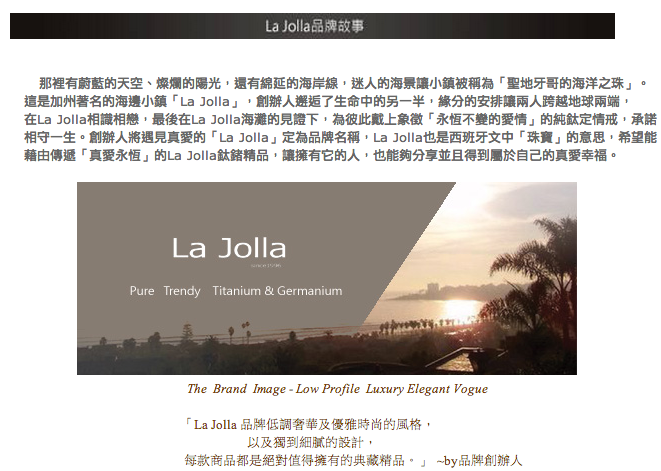
\includegraphics[%
  width=16cm,keepaspectratio]{images/LaJolla}
\caption{\label{fig:LaJolla}LaJolla樂活雅鈦鍺精品}
%(資料來源:本研究整理)
\end{figure}
